\documentclass[12pt, a4paper, addpoints]{exam} % addpoints: 允许在每题后指定分数

% 1. 中文字体和页面设置
\usepackage{xeCJK}
%\usepackage{exam}
\setCJKmainfont{Source Han Serif SC} % 使用思源宋体,请确保系统已安装
\usepackage[inner=2cm, outer=2cm, top=2cm, bottom=2cm]{geometry}
\usepackage{amsmath, amssymb} % 数学公式和符号
\everymath{\displaystyle}
\usepackage{graphicx}
\usepackage{setspace} % 用于设置行距
\everymath{\displaystyle}
% --- 将分值单位改成“分”,并显示为“(10分)” ---
\pointname{分}                % “10分”;若想有空格就写 { 分}
\marginpointname{分}          % 右/左边距里的分值单位(若你用 \pointsinmargin)
\bonuspointname{分}           % 赠分题(如果会用到)
\pointformat{(\thepoints)}    % 题目前显示成 “(10分)”
% -----------------------------------------------


% 2. 自定义作业信息
\def\TitleName{初三数学课后作业 (隐圆与二次函数)}
\def\TeacherName{}
\def\chinesedate{\the\year 年\the\month 月\the\day 日}
\def\ClassName{}

% 3. 页眉和页脚设置
\pagestyle{headandfoot} % 启用 exam 宏包的页眉页脚

% 页眉内容(\small 是为了让字体小一点)
\lhead{\small \TitleName}               % 左页眉:作业名称
\chead{\small 授课教师:\TeacherName}    % 中页眉:教师
%\rhead{\small 成绩:\ClassName}         % 右页眉:班级
\footer{}{\thepage}{}                   % 页脚:只在中间显示页码

% 页眉下方横线和间距
\renewcommand{\headrule}{%
  \hrule height 0.4pt
  \vspace{6pt} % 页眉和正文间距
}


\begin{document}

% 顶部信息和总分
%\noindent\textbf{姓名:\qquad\qquad\qquad\qquad 成绩:\rule{3cm}{0.4pt}}
\vspace{10pt}


%=========================== 题目区 ===========================

\begingroup\setstretch{2.35} % 设置行距为1.35倍行距

\begin{questions}

% --- 题目开始 ---

% 显示为 (10分)
\question[10] 如图,在四边形 $ABCD$ 中,$\angle{ABC}=\angle{D}=90^{o}$,连接 $AC$,点F为 $CD$ 边上一点,
连接 $BE$ 交 $AC$ 于点E,$AB=AE$,$\angle{FGC}+\angle{FBG}=90^{o}$,$\angle{BFG}+2\angle{GFC}=180^{o}$,
若 $AD=\frac{7\sqrt{2}}{2}$,$BG=4$,则$CG$的长为 \rule{3cm}{0.4pt}.

\ \ 
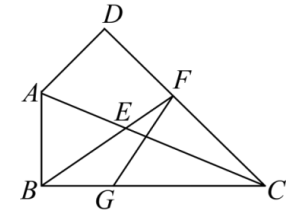
\includegraphics[scale=1]{2222.png}
\vspace{6cm}




% 总分显示为 (15分)
\question[15] 如图,二次函数 $y=-x^2+2mx+2m+1 $ (m是常数,且 $m>0$)的图象与x轴交于A,B两点(点A在点B的
左侧),与y轴交于点C,顶点为D.其对称轴与线段 $BC$ 交于点E,与x轴交于点F.连接 $AC$.若 $\angle{BEF}=2\angle{ACO}$ ,
则m的值是多少?

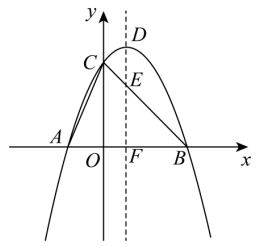
\includegraphics[scale=1]{1111.png}
\vspace{6cm}


(22-23九年级上·龙江哈尔滨·阶段练习)如图,在四边形ABCD中,
$\angle A B C = \angle D = 9 0 ^ { \circ }$ ,连接$A C$ ,点F为边
$C D$ 上点,连接BF交AC于点 $\boldsymbol { E }$ , $A B = A E$
,∠FGC+∠FBG=90°, $\angle B F G + 2 \angle G F C = 1 8 0 ^ { \circ }$ 若
$AD=\frac{7\sqrt{2}} { 2 }$ $BG=4$ ,则CG的长为\_



\vspace{6cm}

10. 如右图,若$\triangle{ABC}\cong\triangle{ADE}$,且$\angle{B}=60^{\circ}$,$\angle{C}=30^{\circ}$,则 cYalowb $\angle D A E = 90 ^ { \circ }$
\vspace{6cm}
%\includegraphics[keepaspectratio]{../qs_image_DB/微信图片_2025-10-18_163036_121/59f62b99551bced135e5c04e0f88afcf1348ebe6b6686416b9f9e823276d5f19.jpg}

【变式1】 函数 $y = { \frac { x - 1 } { x ^ { 2 } - x + 1 } } ( x > 1 )$ 的最大值为

解法1:像这种 $= 10 7 \frac { 1 \times 10 ^ { 3 } k g } { 1 = 1 \times 10 ^ { 3 } k g }$ 型的分式函数,通用做法是令一次函数部分为 $t ,$ 再分子分母同除以 $t ,$ 令 $t = x - 1$ ,则 $t > 0$ , $x = t + 1$ ,所以 $y = \frac { t } { \left( t + 1 \right) ^ { 2 } - \left( t + 1 \right) + 1 } = \frac { t } { t ^ { 2 } + t + 1 } = \frac { 1 } { t + \frac { 1 } { t } + 1 } \leq \frac { 1 } { 2 \sqrt { t \cdot \frac { 1 } { t } } + 1 } = \frac { 1 } { 3 } \ : ,$ 当且仅当 $t = { \frac { 1 } { t } }$ , 即 $t = 1$ 时取等号,此时 $x = 2$ ,故函数 $y = { \frac { x - 1 } { x ^ { 2 } - x + 1 } } ( x > 1 )$ 的最大值为 $\frac 13$ 解法2:把函数的解析式看成关于 $x$ 的方程,将方程变形,利用判别式研究y的最值,将y= $y = { \frac { x - 1 } { x ^ { 2 } - x + 1 } }$ 变形成 $y ( x ^ { 2 } - x + 1 ) = x - 1$ ,整理得: $y x ^ { 2 } - ( y + 1 ) x + y + 1 = 0 \textcircled { 1 } ,$ 当 $y \neq 0$ 时,把 $\textcircled{1}$ 看成关于 $x$ 的一元二次方程,其判别式 $\Delta = [ - ( y + 1 ) ] ^ { 2 } - 4 y ( y + 1 ) \geq 0$ ,解得: $- 1 \leq y \leq \frac { 1 } { 3 }$ ,要得出y的最大值是 $\frac 13$ 还需验证等号能成立,可把 $y = \frac 13$ 代回 $y = { \frac { x - 1 } { x ^ { 2 } - x + 1 } }$ 看能否求出满足题意的 $x ,$ 由 $\frac { 1 } { 3 } = \frac { x - 1 } { { x } ^ { 2 } - x + 1 }$ 可解得: $x = 2$ ,满足 $x > 1$ ,所以函数 $y = { \frac { x - 1 } { x ^ { 2 } - x + 1 } } ( x > 1 )$ 的最大值为 $\frac 13$ 答案: $\frac 13$

\vspace{6cm}

解法1: $\overrightarrow { A C }$ , $\overrightarrow { A E }$ 的长度、夹角都容易计算,故可用定义求数量积,由题意, $\ddot { \varsigma _ { \bf i } } = \sqrt { 4 ^ { 2 } + 3 ^ { 2 } } = 5 , \ \left| \overline { { { A E } } } \right| = \frac { 1 } { 2 } \Big | \overline { { { A B } } } \Big | = 2 , \ \ \overline { { { A C } } } \cdot \overline { { { A E } } } = \Big | \overline { { { A C } } } \Big | \cdot \Big | \overline { { { A E } } } \Big | \cdot \cos \angle C A E = 5 \times 2 \times \frac { \Big | \overline { { { A B } } } \Big | } { \Big | \overline { { { A C } } } \Big | } = 10 \times \frac { 4 } { 5 } = 8 . $



\end{questions}
\endgroup
\end{document}